\chapter{XSS (Cross-Site Scripting)}

Gli attacchi \textit{Cross-Site Scripting} (\textbf{XSS}) sono un tipo di injection, in cui gli
script maligni
vengono iniettati in siti web in realtà benigni e affidabili.
Si verificano quando un aggressore
utilizza un'applicazione web per inviare codice malevolo, generalmente sotto
forma di script
(javascript) lato browser, ad un altro utente finale.
I flaws che permettono a questi attacchi di avere successo sono abbastanza diffusi
e si
verificano ovunque un'applicazione web utilizza l'input di un utente all'interno
dell'output che
genera, senza effettivamente validarlo o codificarlo.
Gli attacchi Cross-Site Scripting si verificano quando:

\begin{itemize}
      \item I dati entrano in un'applicazione web attraverso una fonte non
            attendibile, il più delle
            volte tramite una richiesta web.
      \item I dati sono inclusi in contenuti dinamici che vengono inviati ad un
            utente web senza
            essere convalidati per contenuti dannosi.
\end{itemize}

Il contenuto dannoso inviato al browser web spesso assume la forma di un segmento
di JavaScript, ma può anche includere HTML, Flash o qualsiasi altro tipo di codice
che il browser può eseguire.
La varietà di attacchi basati su XSS è molto vasta, ma comunemente includono:

\begin{itemize}
      \item trasmettere all'aggressore dati privati, come cookies o altre
            informazioni di sessione (password),
      \item Dirigere la vittima a contenuti web controllati dall'aggressore,
      \item Effettuare altre operazioni dannose sulla macchina dell'utente,
            simulando il sito vulnerabile.
\end{itemize}

\newpage

Gli attacchi XSS possono essere generalmente classificati in tre categorie:

\begin{itemize}
      \item \textbf{Stored}
      \item \textbf{Reflected}
      \item \textbf{DOM Based}
\end{itemize}

\section{Attacchi}

\subsection{Stored}

Gli attacchi di tipo \textit{Stored} (memorizzati) sono quelli in cui lo script iniettato viene memorizzato in
modo permanente sui server di destinazione, ad esempio in una banca dati, in un forum di messaggi, nel registro dei visitatori, nel campo dei commenti, ecc.
La vittima recupera quindi lo script dannoso dal server quando richiede le informazioni memorizzate.
Gli XSS memorizzati vengono anche chiamati \textit{XSS Persistenti} o \textit{XSS di tipo I}.

\paragraph{Esempio.}
Prendiamo in esame il seguente schema che rappresenta un attacco che avviene
sfruttando i post dei forum:

\begin{figure}[H]
      \centering
      \includegraphics[width=\textwidth, keepaspectratio]{capitoli/secure_coding/img/cap_9/stored.png}
      \caption{Schema di un attacco XSS Server Stored.}
\end{figure}

\begin{enumerate}
      \item L'attaccante inserisce del codice javascript in un post e questo viene
            automaticamente memorizzato nel database.
      \item La vittima che vuole vedere quel post, ci clicca.
      \item Il commento viene scaricato automaticamente dal database e viene
            visualizzato nel browser dell'utente andando ad eseguire il codice
            javascript al suo interno.
\end{enumerate}

Attacchi di questo tipo possono ad esempio rubare e
fornire all'attaccante il file dei cookie.

\subsection{Reflected}

Gli attacchi \textit{Reflected} (riflessi) sono quelli in cui lo script iniettato viene ``riflesso'' dal server web, ad esempio in un messaggio di errore, in un risultato di ricerca o in qualsiasi altra risposta che
include parte o tutto l'input inviato al server come parte della richiesta.
Gli attacchi riflessi vengono quindi consegnati alle vittime attraverso un'altra via, ad esempio in un
messaggio di posta elettronica o su un altro sito web.
Quando un utente viene ingannato a cliccare su un link maligno, a inviare un modulo appositamente creato o anche solo a navigare su un sito maligno, il codice
iniettato viaggia verso il sito web vulnerabile, che riflette l'attacco al browser dell'utente.
Il browser esegue poi il codice perché proviene da un server ``di fiducia''.
Gli XSS riflessi sono anche chiamati \textit{XSS Non-Persistenti} o \textit{XSS di tipo II}.

\newpage

\paragraph{Esempio ``\textit{Client Reflected}''.}
Analizziamo il seguente schema:

\begin{figure}[H]
      \centering
      \includegraphics[width=\textwidth, keepaspectratio]{capitoli/secure_coding/img/cap_9/xss1.png}
      \caption{Schema di un attacco XSS Client Reflected.}
\end{figure}

\begin{enumerate}
      \item Viene inviato un link ad un utente in qualche modo, per esempio
            tramite email e
            questo viene cliccato.
      \item Viene chiamato il server relativo al link (get al server).
            In questo caso è buono, non è
            malevolo. Nel link è stato inserito un parametro che non è una stringa
            ma uno script.
            Solitamente questo server che stiamo chiamando restituisce una
            pagina contenente la keyword
            cercata con il link
            o un messaggio per l'esito negativo della ricerca.
      \item Il server web vede arrivare la richiesta; il server restituisce una
            risposta visualizzabile
            sul browser. Invece della keyword, rimanda indietro una pagina con il codice
            che
            altro non era che il parametro dell'URL.
      \item Nel nostro caso avevamo codice javascript.
            Viene restituita quindi una pagina e poi...
      \item ...viene eseguito il codice javascript malevolo.
\end{enumerate}

L'attacco viene detto "\textit{reflected}" perché il server web ha riflesso la domanda. Il sito è giusto,
il server web è lecito (fa solo da veicolo), ma la keyword è stata scritta in modo da far eseguire il codice malevolo nel browser.

\subsection{DOM Based}

DOM Based XSS (o, come viene chiamato in alcuni testi, ``\textit{type-0 XSS}'') è un attacco XSS in
cui il payload dell'attacco viene eseguito come risultato della modifica dell'``ambiente'' DOM
nel browser della vittima utilizzato dallo script originale lato client, in modo che il codice
venga eseguito in modo ``inaspettato''.
Il Document Object Model (DOM) è un'interfaccia di programmazione applicativa indipendente dalla piattaforma e dal linguaggio che tratta un documento HTML, XHTML o XML come una struttura ad albero in cui ogni nodo è un oggetto che rappresenta una parte del documento.
Quando una pagina web viene caricata, il browser crea un Document Object Model della pagina, che è una rappresentazione orientata agli oggetti di un documento
HTML, che funge da interfaccia tra JavaScript e il documento stesso e permette la creazione di pagine web dinamiche.

\vspace{-1em}

\begin{figure}[H]
      \centering
      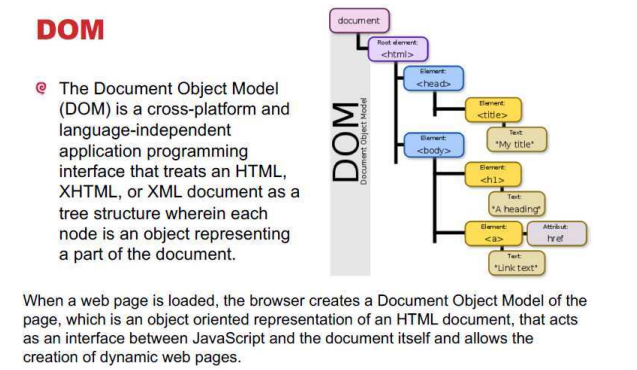
\includegraphics[width=\textwidth, keepaspectratio]{capitoli/secure_coding/img/cap_9/dom.png}
\end{figure}

\vspace{-2em}

\paragraph{Esempio.}
Supponiamo che un codice venga utilizzato per creare un modulo che permetta all'utente di scegliere la lingua preferita. Nella query viene fornita anche una lingua
predefinita, come parametro ``default''.
La pagina viene invocata con un URL. Un attacco contro questa pagina può essere effettuato inviando il seguente URL a una vittima. Quando la vittima clicca su
questo link, il browser invia una certa richiesta. Il server risponde con la pagina contenente il codice Javascript. Il browser crea un oggetto DOM per la pagina, in cui l'oggetto \verb|document.location| contiene la stringa.
Il codice Javascript originale nella pagina non si aspetta che il parametro di default contenga il markup HTML, e come tale lo fa semplicemente echeggiare nella pagina (DOM) a runtime.

\subsection{Un'altra Classificazione}

Secondo la prima classificazione \textbf{Stored}, \textbf{Reflected} e \textbf{DOM Based} sono tre diversi tipi di XSS, ma in realtà questi si sovrappongono. Si possono avere gli DOM Based XSS sia Stored che Reflected. Si possono avere anche Non-DOM Based XSS Stored e Reflected.
Possiamo effettuare un'ulteriore distinzione: \textit{Server Side} o \textit{Client Side}.

\paragraph{Server Side: } si verifica quando i dati forniti dall'utente untrusted sono inclusi in una
risposta HTML generata dal server. La fonte di questi dati potrebbe provenire dalla richiesta o da una posizione stored (memorizzata).
E' possibile avere sia Reflected che Stored Server XSS.
In questo caso, l'intera vulnerabilità è in codice lato server, e il browser sta semplicemente prendendo la risposta ed eseguendo uno script valido incorporato.

\paragraph{Client Side: } si verifica quando i dati forniti dall'utente untrusted vengono utilizzati per
aggiornare il DOM con una chiamata JavaScript che non è sicura. Una chiamata JavaScript è considerata unsafe se può essere utilizzata per introdurre JavaScript
valido nel DOM.
Questa fonte di dati potrebbe provenire dal DOM o potrebbe essere stata inviata dal server (tramite una chiamata AJAX o un page load). La fonte finale dei
dati potrebbe provenire da una richiesta o da una posizione memorizzata sul client o sul server.
È possibile avere sia Reflected che Stored Client XSS.

\section{Mitigation}

Per cercare di arginare questo tipo di problemi possiamo fare riferiamo soprattutto a strumenti per l'individuazione.
\textbf{BlueClosure Detect} può ana\-lizzare qualsiasi codice scritto con framework JavaScript come
\textit{Angular.js}, \textit{jQuery}, \textit{Meteor.js}, \textit{React.js} e molti altri. BlueClosure Detect utilizza un avanzato motore di strumentazione Javascript per capire il codice. Il motore BCD è in grado di ispezionare qualsiasi codice, indipendentemente da quanto sia offuscato.
La tecnologia BlueClosure è in grado di scansionare automaticamente un intero sito web.
Questo è il modo più veloce per scansionare e analizzare GRANDI portali aziendali con ricchi contenuti Javascript come farebbe un tester con il suo browser.
Ci sono poi i tools di \textit{Pentest}: \textbf{Nessus}, \textbf{Nikto}, e alcuni altri strumenti disponibili possono aiutare a scansionare un sito web per questi difetti, ma soltanto superficialmente.
Se una parte di un sito web è vulnerabile, è molto probabile che ci siano anche altri problemi.\\

Per uno sviluppatore web, ci sono due modi diversi di eseguire la gestione sicura degli input:

\begin{itemize}
      \item \textbf{Encoding}, che fa escape all'input dell'utente in modo che il browser lo interpreti solo come dati, non come codice.
      \item \textbf{Validation}, che filtra l'input dell'utente in modo che il browser lo interpreti come codice senza comandi dannosi.
\end{itemize}

Questi metodi condividono caratteristiche comuni, importanti da comprendere
quando si utilizza uno di essi:

\begin{itemize}
      \item \textit{Context Secure}; la gestione degli input deve essere eseguita
            in modo diverso a
            seconda di dove viene inserito l'input dell'utente in una pagina.
      \item \textit{Inbound/Outbound Secure}: la gestione degli input può essere
            effettuata sia quando il
            sito web riceve l'input (in entrata) sia subito prima che il
            sito web
            inserisca l'input in una pagina (in uscita).
      \item \textit{Client/Server Secure}: la gestione degli input può essere
            effettuata sia sul lato client
            che lato server, entrambi necessari in circostanze diverse.
\end{itemize}

\subsection{Gestione input Inbound/Outbound}

La convalida dell'input deve essere eseguita o quando un sito web riceve l'input
(in entrata)
o quando l'input lascia la pagina al server (in uscita).
L'input dell'utente può essere inserito in diversi contesti in una pagina.
Non c'è un modo
semplice per determinare quando l'input dell'utente arriva e in quale contesto sarà
eventualmente inserito. La gestione degli input in uscita (Outbound input handling)
dovrebbe
essere la linea di difesa primaria contro XSS, in quanto può tenere conto del
contesto
specifico in cui l'input dell'utente verrà inserito.
Nella maggior parte delle moderne applicazioni web, l'input dell'utente viene
gestito sia dal
codice lato server che dal lato client.
Al fine di proteggere da XSS tradizionali, la gestione sicura degli input deve
essere
eseguita nel codice lato server. Questo viene fatto utilizzando qualsiasi linguaggio
supportato dal server. Invece, per proteggersi da XSS basati su DOM in cui il
server non riceve mai la stringa
dannosa, la gestione sicura degli input deve essere eseguita nel codice lato client.
Questo viene fatto utilizzando JavaScript.

\newpage

\subsection{XSS Prevention Cheat Sheet}

Vediamo ora una lista di suggerimenti utili per prevenire attacchi XSS.

\vspace{-0.5em}

\paragraph{Rule \#0:} non inserire mai dati non attendibili, se non in posizioni
consentite.
La prima regola è quella di negare tutto (deny all), non inserire dati non
attendibili nel documento HTML a meno che non si trovino all'interno di uno degli
slot definiti dalla Rule \#0 alla Rule \#4.

\vspace{-0.5em}

\paragraph{Rule \#1:} : \textit{effettuare \textbf{escaping} del codice HTML
      prima di inserire dati non attendibili nell'HTML}.
La Rule \#1 è per quando si desidera inserire dati non attendibili da qualche
parte
direttamente nel corpo HTML. Questo include all'interno di normali tag come
\verb|div|, \verb|p|, \verb|b|, \verb|td|,
ecc. La maggior parte dei framework web hanno un metodo per l'escape dell'HTML
per i caratteri descritti di seguito.

\begin{itemize}
      \item \verb|&| $\rightarrow$ \verb|&amp;|
      \item \verb|<| $\rightarrow$ \verb|&lt;|
      \item \verb|>| $\rightarrow$ \verb|&gt;|
      \item \verb|"| $\rightarrow$ \verb|&quot;|
      \item \verb|'| $\rightarrow$ \verb|&#x27;| o \verb|&apos;|. Quest'ultimo
            non è raccomandato in quanto non è tra i caratteri presenti in HTML, ma si trova
            tra quelli di XML e XHTML.
      \item \verb|/| $\rightarrow$ \verb|&#x2F;|
\end{itemize}

\vspace{-0.5em}

\paragraph{Rule \#2:} \textit{escaping degli attributi prima di inserire dati non
      attendibili negli attributi comuni HTML}.
Regola per inserire dati non attendibili in valori tipici degli attributi come
larghezza, nome,
valore, ecc. Questo non dovrebbe essere usato per attributi complessi come
\verb|href|, \verb|src|, \verb|style|,
o qualsiasi gestore di eventi come \verb|onmouseover|.

\vspace{-0.5em}

\paragraph{Rule \#3:} \textit{javascript escape prima di inserire dati non attendibili
      nei valori dei dati javascript}.
Riguarda il codice JavaScript generato dinamicamente.

\vspace{-0.5em}

\paragraph{Rule \#4:} \textit{css escape e validare rigorosamente prima di inserire
      dati non attendibili nei valori delle proprietà di stile HTML}.
Sempre validare ed effettuare l'escaping quando si desidera inserire dati non
attendibili in un foglio di stile o in un
tag di stile. I CSS
sono sorprendentemente potenti e possono essere utilizzati per numerosi attacchi.

\subsection{Validazione}

L'encoding da solo non basta.
La validazione è l'atto di filtrare l'input dell'utente in modo che tutte le
parti dannose di esso
siano rimosse, senza necessariamente rimuovere tutto il codice in esso contenuto.
Uno dei
tipi di validazione più riconoscibili nello sviluppo web è quello che permette
alcuni elementi
HTML, come \verb|<em>| e \verb|<strong>|, ma ne esclude altri come \verb|<script>|.